\documentclass[aspectratio=169]{beamer}
% \usepackage{pgfpages}
% \pgfpagesuselayout{4 on 1}[a4paper,landscape,border shrink=5mm]
\usepackage{tikz}
\usetikzlibrary{shapes, backgrounds, arrows, positioning}
%\usepackage{pgfplots}
\usepackage{listings}
\usepackage[utf8,latin1]{inputenc}
\usepackage[style = apa, backend = biber, natbib = true]{biblatex}
\addbibresource{../../literature/lit.bib}

\makeatletter \def\newblock{\beamer@newblock} \makeatother  

\beamertemplatenavigationsymbolsempty
\setbeamertemplate{itemize items}[circle]
\setbeamertemplate{section in toc}[circle]
\mode<beamer>{\setbeamercolor{math text displayed}{fg=iwmgray}}
\setbeamercolor{block body}{bg=iwmorange!50!white}
\setbeamercolor{block title}{fg=white, bg=iwmorange}

% Definitions for biblatex
\setbeamercolor{bibliography entry note}{fg=iwmgray}
\setbeamercolor{bibliography entry author}{fg=iwmgray}
\setbeamertemplate{bibliography item}{}


\definecolor{iwmorange}{RGB}{255,105,0}
\definecolor{iwmgray}{RGB}{67,79,79}
\definecolor{iwmblue}{RGB}{60,180,220}
\definecolor{iwmgreen}{RGB}{145,200,110}
\definecolor{iwmpurple}{RGB}{120,0,75}

\setbeamercolor{title}{fg=iwmorange}
\setbeamercolor{frametitle}{fg=iwmorange}
\setbeamercolor{structure}{fg=iwmorange}
\setbeamercolor{normal text}{fg=iwmgray}
\setbeamercolor{author}{fg=iwmgray}
\setbeamercolor{date}{fg=iwmgray}

\title{Crossed random effects}
\author{Nora Wickelmaier}
\date{Last modified: \today}

\newcommand{\vect}[1]{\mathbf{#1}}
\newcommand{\mat}[1]{\mathbf{#1}}
\newcommand{\gvect}[1]{\boldsymbol{#1}}
\newcommand{\gmat}[1]{\boldsymbol{#1}}

\lstset{language = R,%
  basicstyle = \ttfamily\color{iwmgray},
  frame = single,
  rulecolor = \color{iwmgray},
  commentstyle = \slshape\color{iwmgreen},
  keywordstyle = \bfseries\color{iwmgray},
  identifierstyle = \color{iwmpurple},
  stringstyle = \color{iwmblue},
  numbers = none,%left,numberstyle = \tiny,
  basewidth = {.5em, .4em},
  showstringspaces = false,
  emphstyle = \color{red!50!white}}

\pgfmathdeclarefunction{gauss}{2}{%
  \pgfmathparse{1/(#2*sqrt(2*pi))*exp(-((x-#1)^2)/(2*#2^2))}%
}

\AtBeginSection[]{
  \frame{
    \tableofcontents[sectionstyle=show/hide, subsectionstyle=show/show/hide]}}

\setbeamertemplate{headline}{
 \begin{beamercolorbox}{section in head}
   \vskip5pt\insertsectionnavigationhorizontal{\paperwidth}{}{}\vskip2pt
 \end{beamercolorbox}
}

\setbeamertemplate{footline}{\vskip-2pt\hfill\insertframenumber$\;$\vskip2pt}

\begin{document}

\begin{frame}{}
\thispagestyle{empty}
\titlepage
\end{frame}

% \begin{frame}{Outline}
% \tableofcontents
% \end{frame}

\begin{frame}{Crossed random effects}
  \begin{itemize}
    % \item Crossed random effects are fitted for cross-classified data (each
    %   level of one factor is crossed with each level of the other factor)
    \item In many experiments in psychology the reaction of each subject ($j =
      1, \dots, N$) to a complete set of stimuli or items ($k = 1, \dots, K$) is
      measured
  \[
    y_{ijk} = \beta_0 + \beta_ix_{i} + \upsilon_{0j} + \eta_{0k} + \varepsilon_{ijk}
  \]
  with $\varepsilon_{ijk} \overset{iid}{\sim} N(0,\sigma^2)$, 
  $\upsilon_{0j} \overset{iid}{\sim} N(0,\sigma^2_{\upsilon})$, and 
  $\eta_{0k} \overset{iid}{\sim} N(0,\sigma^2_{\eta})$

    \item Data are completely crossed: all subjects are presented with all items
  \end{itemize}
  \footnotesize
  \begin{center}
  \begin{tabular}{lcccccc}
    & & \multicolumn{5}{c}{Subject}\\
    \cline{3-7}
     & & 1 & 2 & 3 & \dots & 20 \\
    \hline
      & 1 & $1$ & $1$ & $1$ & \dots & $1$ \\
      & 2 & $1$ & $1$ & $1$ & \dots & $1$ \\
Item  & 3 & $1$ & $1$ & $1$ & \dots & $1$ \\
      & \vdots & \vdots & \vdots & \vdots & \vdots & \vdots\\
      & 10 & $1$ & $1$ & $1$ & \dots & $1$ \\
      \hline
  \end{tabular}
  \end{center}
\end{frame}

\begin{frame}[fragile]{Crossed random effects}
  \vspace{-.6cm}
  \begin{columns}
    \begin{column}[t]{4.5cm}
  \begin{lstlisting}
> head(dat, 12)
   id  cond   item  av
1   1 cond1 item01 105
2   1 cond1 item02 116
3   1 cond1 item03 104
4   1 cond1 item04  81
5   1 cond1 item05  99
6   1 cond1 item06 109
7   1 cond1 item07 100
8   1 cond1 item08 103
9   1 cond1 item09  89
10  1 cond1 item10  94
11  2 cond1 item01 107
12  2 cond1 item02 100
  \end{lstlisting}
    \end{column}

    \begin{column}[t]{7cm}
  \begin{lstlisting}
> xtabs( ~ item + id, dat)
        id
item     1 2 3 4 5 6 7 8 9 ... 20
  item01 1 1 1 1 1 1 1 1 1 ...  1
  item02 1 1 1 1 1 1 1 1 1 ...  1
  item03 1 1 1 1 1 1 1 1 1 ...  1
  item04 1 1 1 1 1 1 1 1 1 ...  1
  item05 1 1 1 1 1 1 1 1 1 ...  1
  item06 1 1 1 1 1 1 1 1 1 ...  1
  item07 1 1 1 1 1 1 1 1 1 ...  1
  item08 1 1 1 1 1 1 1 1 1 ...  1
  item09 1 1 1 1 1 1 1 1 1 ...  1
  item10 1 1 1 1 1 1 1 1 1 ...  1
  \end{lstlisting}
    \end{column}
  \end{columns}
\end{frame}

\section{Lexical decision task}

\begin{frame}[<+->]{Lexical decision task \citep{Baayen2008}}
  \begin{itemize}
    \item This example will show how to include subjects and items as
      crossed, independent, random effects, as opposed to hierarchical or
      multilevel models in which random effects are assumed to be nested
    \item Assume an example data set with three participants s1, s2 and s3
      who each saw three items w1, w2, w3 in a priming lexical decision
      task under both short and long stimulus onset asynchrony (SOA) conditions
    \item The data are generated by the following model with random intercepts
      for subject and item, and random slopes for subject
  \[
    y_{ijk} = \beta_0 + \beta_1 SOA_k + \omega_{0j} + \upsilon_{0i} +
      \upsilon_{1i} SOA_k + \varepsilon_{ijk} 
  \]
\small
with $\gvect{\upsilon} \sim N\left(\gvect{0}, \gmat{\Sigma}_{\upsilon} = 
    \begin{pmatrix}
      \sigma^2_{\upsilon_0} & \sigma_{\upsilon_0\upsilon_1} \\
      \sigma_{\upsilon_0\upsilon_1} & \sigma^2_{\upsilon_1} \\
    \end{pmatrix}\right)$,
      $\omega_{0j} \sim N(0, \sigma_{\omega}^2)$, $\varepsilon_{ijk} \sim N(0,
  \sigma_{\varepsilon}^2)$, all i.i.d. 
  \end{itemize}
\end{frame}

\begin{frame}{Structure of the data set}
  \begin{columns}
    \begin{column}{.4\textwidth}
      \centering
  \scriptsize
  \begin{tabular}{llll}
    \hline
    Subj & Item & SOA & RT  \\
    \hline
    s1 & w1 & Long  & 466 \\
    s1 & w2 & Long  & 520 \\
    s1 & w3 & Long  & 502 \\
    s1 & w1 & Short & 475 \\
    s1 & w2 & Short & 494 \\
    s1 & w3 & Short & 490 \\
    s2 & w1 & Long  & 516 \\
    s2 & w2 & Long  & 566 \\
    s2 & w3 & Long  & 577 \\
    s2 & w1 & Short & 491 \\
    s2 & w2 & Short & 544 \\
    s2 & w3 & Short & 526 \\
    s3 & w1 & Long  & 484 \\
    s3 & w2 & Long  & 529 \\
    s3 & w3 & Long  & 539 \\
    s3 & w1 & Short & 470 \\
    s3 & w2 & Short & 511 \\
    s3 & w3 & Short & 528 \\
    \hline
  \end{tabular}
    \end{column}
    \begin{column}{.6\textwidth}
      \begin{itemize}
        \item When we collect data, we might get a data set like this
        \item We fit a model to the data to separate the structural and the
          stochastical parts
      \end{itemize}
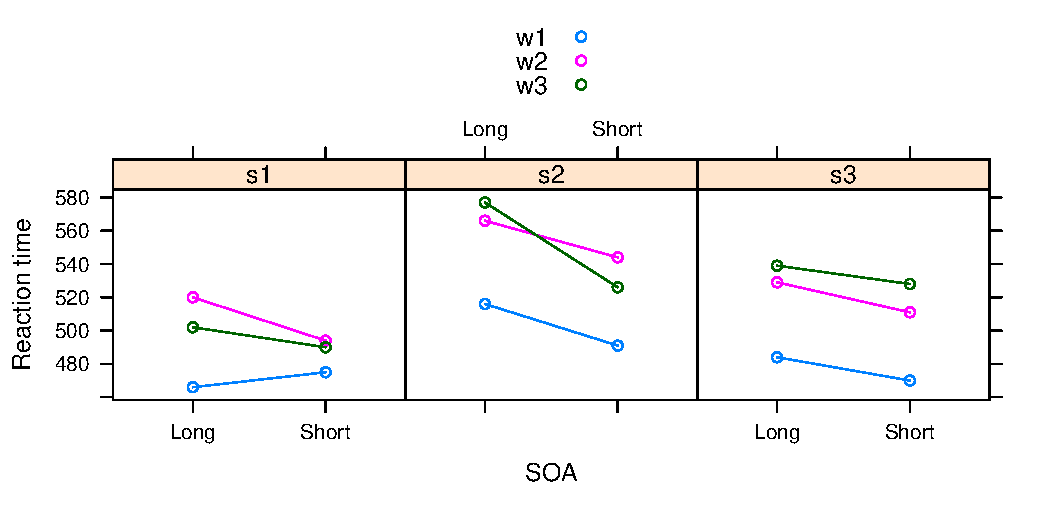
\includegraphics[scale=.5]{../figures/baayen_ex}
    \end{column}
  \end{columns}
\end{frame}

\begin{frame}{Aggregated data}
  \begin{center}
    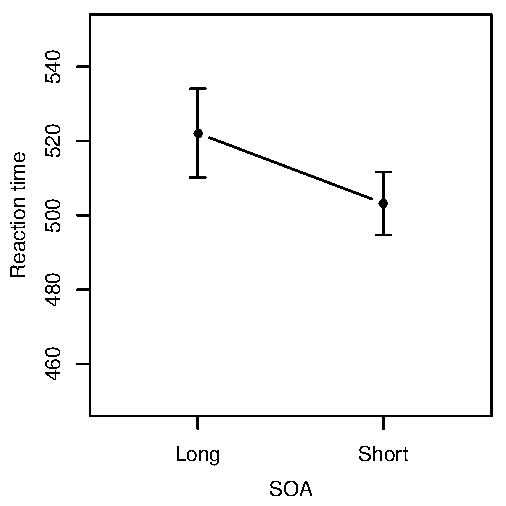
\includegraphics[scale=.8]{../figures/baayen_ex_agg}
  \end{center}
\end{frame}

\begin{frame}{Structure of the data set}
  \vspace{.2cm}
  \scriptsize
  \centering
  \begin{tabular}{llllcrrrcr}
    \hline
    Subj & Item & SOA & RT & Fixed &&  Random &&& Res \\
    \cline{5-6}
    \cline{7-10}
    & & & & Int & SOA & ItemInt & SubInt & SubSOA & \\
    \hline
    s1 & w1 & Long  & 466 & 522.2 & 0     & $-$28.3 & $-$26.2 & 0       & $-$2.0 \\
    s1 & w2 & Long  & 520 & 522.2 & 0     & 14.2    & $-$26.2 & 0       & 9.8 \\
    s1 & w3 & Long  & 502 & 522.2 & 0     & 14.1    & $-$26.2 & 0       & $-$8.2 \\
    s1 & w1 & Short & 475 & 522.2 & $-$19 & $-$28.3 & $-$26.2 & 11      & 15.4 \\
    s1 & w2 & Short & 494 & 522.2 & $-$19 & 14.2    & $-$26.2 & 11      & $-$8.4 \\
    s1 & w3 & Short & 490 & 522.2 & $-$19 & 14.1    & $-$26.2 & 11      & $-$11.9 \\
    s2 & w1 & Long  & 516 & 522.2 & 0     & $-$28.3 & 29.7    & 0       & $-$7.4 \\
    s2 & w2 & Long  & 566 & 522.2 & 0     & 14.2    & 29.7    & 0       & 0.1 \\
    s2 & w3 & Long  & 577 & 522.2 & 0     & 14.1    & 29.7    & 0       & 11.5 \\
    s2 & w1 & Short & 491 & 522.2 & $-$19 & $-$28.3 & 29.7    & $-$12.5 & $-$1.5 \\
    s2 & w2 & Short & 544 & 522.2 & $-$19 & 14.2    & 29.7    & $-$12.5 & 8.9 \\
    s2 & w3 & Short & 526 & 522.2 & $-$19 & 14.1    & 29.7    & $-$12.5 & $-$8.2 \\
    s3 & w1 & Long  & 484 & 522.2 & 0     & $-$28.3 & $-$3.5  & 0       & $-$6.3 \\
    s3 & w2 & Long  & 529 & 522.2 & 0     & 14.2    & $-$3.5  & 0       & $-$3.5 \\
    s3 & w3 & Long  & 539 & 522.2 & 0     & 14.1    & $-$3.5  & 0       & 6.0 \\
    s3 & w1 & Short & 470 & 522.2 & $-$19 & $-$28.3 & $-$3.5  & 1.5     & $-$2.9 \\
    s3 & w2 & Short & 511 & 522.2 & $-$19 & 14.2    & $-$3.5  & 1.5     & $-$4.6 \\
    s3 & w3 & Short & 528 & 522.2 & $-$19 & 14.1    & $-$3.5  & 1.5     & 13.2 \\
    \hline
    &&&&&& $\sigma^2_{\omega_0}$ & $\sigma^2_{\upsilon_0}$ &
    $\sigma^2_{\upsilon_1}$ & $\sigma^2_{\varepsilon}$\\ 
    &&&&&&  & \multicolumn{2}{c}{$\sigma_{\upsilon_0\upsilon_1}$} & 
  \end{tabular}
\end{frame}

\begin{frame}{True values}
  \begin{itemize}
    \item We assume the following true parameters for a data simulation
    \vspace{.2cm}
  \begin{center}
  \begin{tabular}{lrr}
    \hline
    Parameter && Model \\
    \hline
    $\beta_0$                     && 522.11\\
    $\beta_1$                     && $-$18.89\\
    $\sigma_{\omega}$             && 21.10\\
    $\sigma_{\upsilon_0}$         && 23.89\\
    $\sigma_{\upsilon_1}$         && 9.00\\
    $\rho_{\upsilon_0\upsilon_1}$ && $-$1.00\\
    $\sigma_{\varepsilon}$        && 9.90\\
    \hline
  \end{tabular}
  \end{center}
     \[
       y_{ijk} = \beta_0 + \beta_1 SOA_k + \omega_{0j} + \upsilon_{0i} +
       \upsilon_{1i} SOA + \varepsilon_{ijk} 
  \]
\small
with $\gvect{\upsilon} \sim N\left(\gvect{0}, \gmat{\Sigma}_{\upsilon} = 
    \begin{pmatrix}
      \sigma^2_{\upsilon_0} & \sigma_{\upsilon_0\upsilon_1} \\
      \sigma_{\upsilon_0\upsilon_1} & \sigma^2_{\upsilon_1} \\
    \end{pmatrix}\right)$,
  $\omega_{0j} \sim N(0, \sigma_{\omega}^2)$, $\varepsilon_{ijk} \sim N(0,
  \sigma_{\varepsilon}^2)$ 
  \end{itemize}
\end{frame}

\begin{frame}[fragile]{Fixed effects}
  \begin{lstlisting}
datsim <- expand.grid(subject = factor(c("s1", "s2", "s3")),
                      item = factor(c("w1", "w2", "w3")),
                      soa = factor(c("long", "short")))
datsim <- datsim |> sort_by( ~ subject)

# model matrix in dummy coding
model.matrix(~ soa, datsim)

beta0 <- 522.11
beta1 <- -18.89
b0 <- rep(beta0, 18)
b1 <- rep(rep(c(0, beta1), each = 3), 3)
cbind(b0, b1)
  \end{lstlisting}
\end{frame}

\begin{frame}[fragile]{Random effects}
  \begin{lstlisting}
sw  <- 21.1
sy0 <- 23.89; sy1 <- 9; ry <- -1
se  <- 9.9

w  <- rep(rnorm(3, mean = 0, sd = sw), 6)
e  <- rnorm(18, mean = 0, sd = se)
# draw from bivariate normal distribution
sig <- matrix(c(sy0^2, ry * sy0 * sy1, ry * sy0 * sy1, sy1^2), 2, 2)
y01 <- mvtnorm::rmvnorm(3, mean = c(0, 0), sigma = sig)
y0 <- rep(y01[,1], each = 6)
y1 <- rep(c(0, y01[1,2],
            0, y01[2,2],
            0, y01[3,2]), each = 3)
cbind(w, y0, y1, e)
  \end{lstlisting}
\end{frame}

\begin{frame}[fragile]{Simulate data}
  \begin{lstlisting}
datsim$rt <- b0 + b1 + w + y0 + y1 + e

# fit model
library(lme4)

lme1 <- lmer(rt ~ soa + (1 | item) + (soa | subject), datsim)
summary(lme1)
confint(lme1)

# btw
?pvalues
?convergence
  \end{lstlisting}
\end{frame}

\begin{frame}{Comparison of sample and model estimates}
  For this example, we are able to compare the ``true'' values to the
  parameter estimates
  \begin{center}
  \begin{tabular}{lrrrr}
    \hline
    Parameter && Sample && Model \\
    \hline
    $\hat\beta_0$ && 522.2 && 522.11\\
    $\hat\beta_1$ && $-$19.00 && $-$18.89\\
    $\hat\sigma_{\omega}$ && 20.59 && 21.10\\
    $\hat\sigma_{\upsilon_0}$ && 23.62 && 23.89\\
    $\hat\sigma_{\upsilon_1}$ && 9.76 && 9.00\\
    $\hat\rho_{\upsilon_0\upsilon_1}$ && $-$0.71 && $-$1.00\\
    $\hat\sigma_{\varepsilon}$ && 8.55 && 9.90\\
    \hline
  \end{tabular}
  \end{center}
     \[
       y_{ijk} = \beta_0 + \beta_1 SOA_k + \omega_{0j} + \upsilon_{0i} +
       \upsilon_{1i} SOA_k + \varepsilon_{ijk} 
  \]
\small
with $\gvect{\upsilon} \sim N\left(\gvect{0}, \gmat{\Sigma}_{\upsilon} = 
    \begin{pmatrix}
      \sigma^2_{\upsilon_0} & \sigma_{\upsilon_0\upsilon_1} \\
      \sigma_{\upsilon_0\upsilon_1} & \sigma^2_{\upsilon_1} \\
    \end{pmatrix}\right)$,
  $\omega_{0j} \sim N(0, \sigma_{\omega}^2)$, $\varepsilon_{ijk} \sim N(0,
  \sigma_{\varepsilon}^2)$ 
\end{frame}


\begin{frame}{Linear mixed-effects model}
  \begin{itemize}
    \item The linear mixed-effects model has the general form
\[
  \vect{y}_i = \mat{X}_i \, \gvect{\beta} + \mat{Z}_i \, \gvect{\upsilon}_i +
               \gvect{\varepsilon}_i
\]
with fixed effects $\gvect{\beta}$, random effects
$\gvect{\upsilon}_i$, and the design matrices $\mat{X}_i$ and $\mat{Z}_i$
  and the assumptions
\[
  \gvect{\upsilon}_i \sim N(\vect{0}, \, \gmat{\Sigma}_\upsilon)
    \text{ i.i.d.}, \qquad
  \gvect{\varepsilon}_i \sim N(\vect{0}, \, \sigma^2 \mat{I}_{n_i})
    \text{ i.i.d.}
\]
  \end{itemize}
\end{frame}

\begin{frame}[shrink=10]{Linear mixed-effects model}
\vspace{2cm}
\begin{equation*}
  \begin{pmatrix}
    y_1 \\
    y_2 \\
    y_3 \\
    \vdots \\
    y_N
  \end{pmatrix} = 
  \begin{pmatrix}
    1 & x_{11} & x_{12} & \dots & x_{1p} \\
    1 & x_{21} & x_{22} & \dots & x_{2p} \\
    1 & x_{31} & x_{32} & \dots & x_{3p} \\
    \vdots & \vdots & \vdots & \vdots & \vdots \\
    1 & x_{N1} & x_{N2} & \dots & x_{Np} \\
  \end{pmatrix} \cdot
  \begin{pmatrix}
    \beta_0 \\
    \beta_1 \\
    \vdots \\
    \beta_p
  \end{pmatrix} +
  \begin{pmatrix}
    z_{10} & z_{11} & \dots & z_{1q} & \dots \\
    z_{20} & z_{21} & \dots & z_{2q} & \dots \\
    z_{30} & z_{31} & \dots & z_{3q} & \dots \\
    \vdots & \vdots & \vdots & \vdots & \vdots \\
    z_{N0} & z_{N1} & \dots & z_{Nq} & \dots \\
  \end{pmatrix} \cdot
  \begin{pmatrix}
    \upsilon_{10} \\
    \vdots \\
    \upsilon_{1q}\\
    \upsilon_{20} \\
    \vdots \\
    \upsilon_{Nq}
  \end{pmatrix} + 
  \begin{pmatrix}
    \varepsilon_1 \\
    \varepsilon_2 \\
    \varepsilon_3 \\
    \vdots \\
    \varepsilon_N
  \end{pmatrix}
\end{equation*}
\end{frame}


\begin{frame}[fragile]{Simulate data using model matrices}
  \begin{lstlisting}
X <- model.matrix( ~ soa, datsim)
Z <- model.matrix( ~ 0 + item + subject + subject:soa, datsim,
  contrasts.arg = 
    list(subject = contrasts(datsim$subject, contrasts = FALSE)))

# fixed effects
beta  <- c(beta0, beta1)

# random effects
u <- c(w = unique(w),
       y0 = y01[,1],
       y1 = y01[,2])

datsim$rt2 <- X %*% beta + Z %*% u + e
  \end{lstlisting}
\end{frame}

\begin{frame}[fragile]{}
  \begin{block}{Exercise}
    \begin{itemize}
      \item Change the data simulation from the previous slides for $N =
        30$ subjects instead of only 3
      \item You can choose if you want to use model matrices or create
        the vectors ``manually''
    \end{itemize}
  \end{block}
  \nocite{Wickelmaier2022}
\end{frame}

\begin{frame}{Summary}
  \begin{itemize}
    \item Mixed-effects model with crossed random effects allow to include
      random effects from different sources (e.\,g., subjects and items)
    \item These models have more power than models on aggregated data like
      ANOVAs or a paired $t$ test in this example \citep[see
      e.\,g.,][]{Jaeger2008}
    \item But more importantly (IMHO), they allow us to assume a much more
      flexible data generating process that seems to be closer to reality
  \end{itemize}
  \vfill
\end{frame}

\section[Physical healing]{Physical healing as a function of perceived time}

\begin{frame}{Physical healing \citep{Aungle2023}}
  \begin{itemize}
    \item \citet{Aungle2023} investigate how perceived time influences physical
      healing
    \item They used cupping to induce bruises on 33 subjects, then took a
      picture, waited for 28\,min and took another picture
    \item Subjects participated in all three conditions over a two week period
    \item Subjective time was manipulated to feel like 14, 28, or 56\,min
    \item The pre and post pictures were presented to 25 raters who rated the
      amount of healing on a 10-point-scale with 0~=~not at all healed,
      5~=~somewhat healed, 10~=~completely healed
  \end{itemize}
  \begin{center}
  \begin{tabular}{l|cccc}
    \hline
    Condition & Mean  & SD    & $N_{subjects}$ & $N_{ratings}$ \\
    \hline
    14-min    & 6.17  & 2.59  & 32             &  800 \\
    28-min    & 6.43  & 2.54  & 33             &  825 \\
    56-min    & 7.30  & 2.25  & 32             &  800 \\
    \hline
  \end{tabular}
  \end{center}
\end{frame}

\begin{frame}{Visualization of data}
  \begin{columns}
    \begin{column}[t]{.6\textwidth}
      Subjects\\
  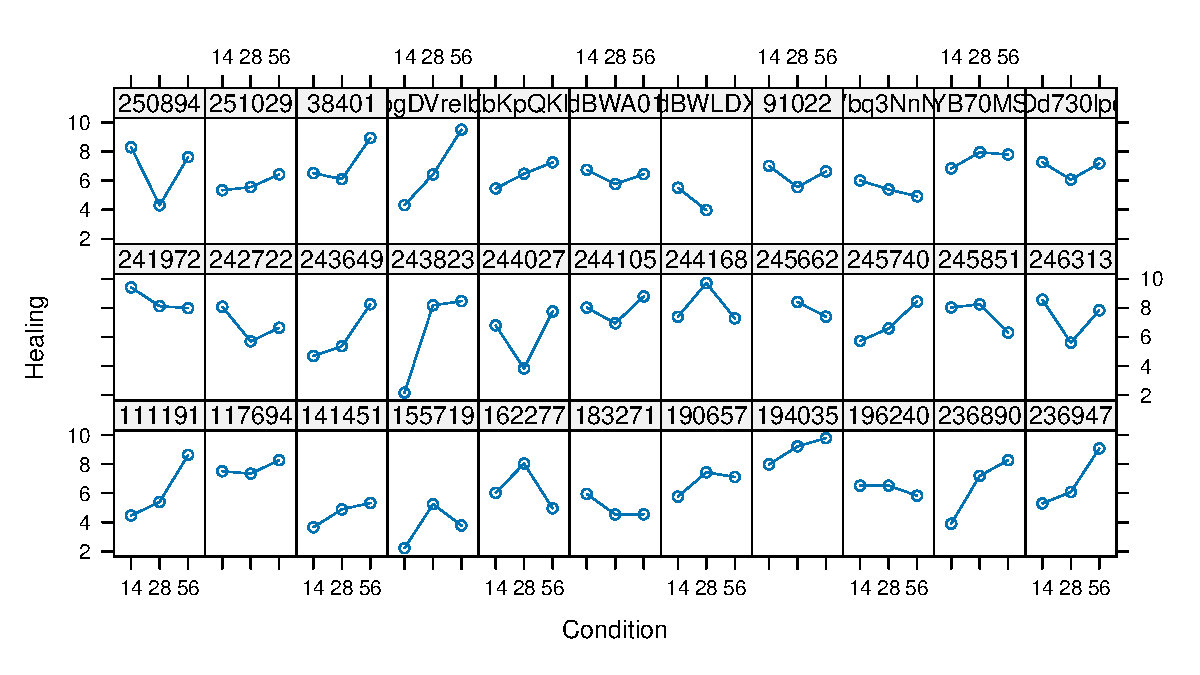
\includegraphics[scale=.45]{../figures/heal_subjects}
    \end{column}

    \begin{column}[t]{.45\textwidth}
      Raters\\
  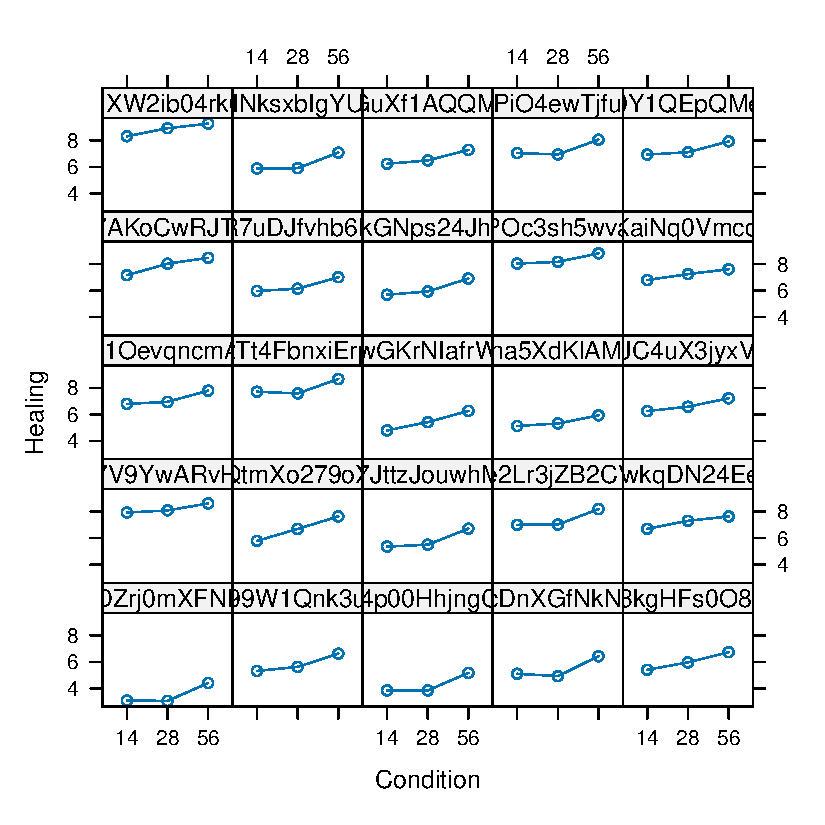
\includegraphics[scale=.45]{../figures/heal_raters}
    \end{column}
  \end{columns}
  \pause
  What model would you choose?
\end{frame}

\begin{frame}{Aggregated data}
  \begin{center}
    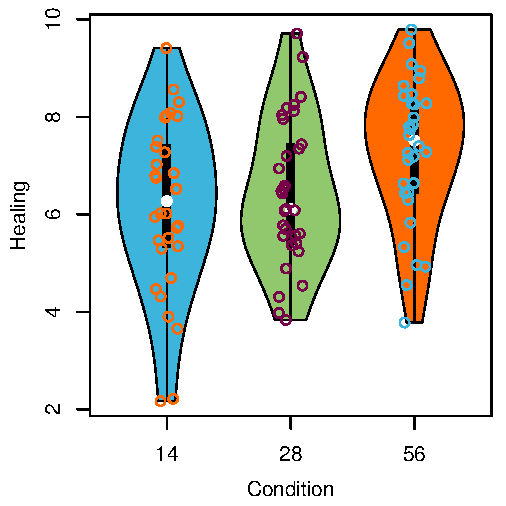
\includegraphics[scale=.8]{../figures/heal_vioplot}
  \end{center}
\end{frame}

\begin{frame}[fragile]{Fitted model}
  \begin{columns}
    \begin{column}{.5\textwidth}
    In the paper, a mixed-effects model with random intercepts for subjects and
      raters was fitted to the data
     \[
       y_{ijk} = \beta_0 + \beta_{1k} Condition_k + \omega_{0j} + \upsilon_{0i} +
       \varepsilon_{ijk}
  \]
\small
      with $\upsilon_{0i} \sim N(0, \sigma_{\upsilon}^2)$,
  $\omega_{0j} \sim N(0, \sigma_{\omega}^2)$, $\varepsilon_{ijk} \sim N(0,
  \sigma_{\varepsilon}^2)$, all i.i.d. 
    \end{column}
    \begin{column}{.5\textwidth}
\begin{tabular}{rrrr}
  \hline
 & Est. & Std. & t value \\ 
  \hline
(Intercept) & 6.20 & 0.32 & 19.56 \\ 
  Condition28 & 0.23 & 0.09 & 2.44 \\ 
  Condition56 & 1.05 & 0.09 & 11.10 \\ 
   \hline
   Random effects & & & \\
   \hline
   Residual & 1.873 & & \\
   Subj (Intercept) & 1.079 & & \\
   Rater (Intercept) & 1.233 & & \\
   \hline
\end{tabular}
    \end{column}
  \end{columns}
  \vspace{.5cm}
\begin{lstlisting}
load("data/healing.RData")
dat <- DFmodel

m1 <- lmer(Healing ~ Condition + (1 | Subject) + (1 | ResponseId), dat)
\end{lstlisting}
\end{frame}

\begin{frame}[<+->]{Selection of random effects}
  \begin{itemize}
    \item How to choose an appropriate random effects structure for a
      mixed-effects model is widely discussed in the literature
      \citep[e.\,g.,][]{Barr2013, Gelman2024, Bates2018}
    \item A prominent view is, that the random effects structure needs to
      represent the experimental design
    \item In our example here, leaving out random slopes for the subjects
      implies that there are no individual effects for subjects
    \item Hence, it is assumed that the experimental manipulation has the same
      effect for every subject
    \item What about the raters in this example? Could they be influenced by
      the conditions?
  \end{itemize}
\end{frame}

\begin{frame}[fragile]{Random slope model}
  \begin{itemize}
    \item Let us add a random slope to the model
\begin{lstlisting}
m2 <- lmer(Healing ~ Condition + (1 + Condition | Subject) +
           (1 | ResponseId), dat)
\end{lstlisting}
\pause
    \item What will change?
\pause
    \item What could be the problem with this model?
  \end{itemize}
\end{frame}

\begin{frame}[<+->]{(Some) Possible models}
  \small
  \begin{itemize}
    \item Model with random intercepts for subjects and random intercepts for
      raters
  \[
    y_{ij} = \beta_0 + \beta_1 Condition_{28} + \beta_2 Condition_{56} +
      \omega_{0j} + \upsilon_{0i} + \varepsilon_{ij} 
  \]
\small
      with $\upsilon_{0i} \sim N(0, \sigma_{\upsilon}^2)$,
      $\omega_{0j} \sim N(0, \sigma_{\omega}^2)$, $\varepsilon_{ij} \sim N(0,
  \sigma_{\varepsilon}^2)$, all i.i.d. 
    \item Model with random slopes for subjects and random intercepts for
      raters
  \[
    y_{ij} = \beta_0 + \beta_1 Condition_{28} + \beta_2 Condition_{56} +
      \omega_{0j} + \upsilon_{0i} + \upsilon_{1i} Condition_{28} +
      \upsilon_{2i} Condition_{56} + \varepsilon_{ij} 
  \]
\small
with $\gvect{\upsilon} \sim N\left(\gvect{0}, \gmat{\Sigma}_{\upsilon} = 
    \begin{pmatrix}
      \sigma^2_{\upsilon_0} & \sigma_{\upsilon_0\upsilon_1}  & \sigma_{\upsilon_0\upsilon_2}\\
      \sigma_{\upsilon_0\upsilon_1} & \sigma^2_{\upsilon_1}  & \sigma_{\upsilon_1\upsilon_2}\\
      \sigma_{\upsilon_0\upsilon_2} & \sigma_{\upsilon_1\upsilon_2} & \sigma^2_{\upsilon_2} \\
    \end{pmatrix}\right)$,
      $\omega_{0j} \sim N(0, \sigma_{\omega}^2)$, $\varepsilon_{ij} \sim N(0,
  \sigma_{\varepsilon}^2)$, all i.i.d. 
    \item Model with random slope for subjects and random intercepts for
      raters, zero correlations
  \[
    y_{ij} = \beta_0 + \beta_1 Condition_{28} + \beta_2 Condition_{56} +
      \omega_{0j} + \upsilon_{0i} + \upsilon_{1i} Condition_{28} +
      \upsilon_{2i} Condition_{56} + \varepsilon_{ij} 
  \]
\small
with $\gvect{\upsilon} \sim N\left(\gvect{0}, \gmat{\Sigma}_{\upsilon} = 
    \begin{pmatrix}
      \sigma^2_{\upsilon_0} & 0  & 0\\
      0 & \sigma^2_{\upsilon_1}  & 0\\
      0 & 0 & \sigma^2_{\upsilon_2} \\
    \end{pmatrix}\right)$,
      $\omega_{0j} \sim N(0, \sigma_{\omega}^2)$, $\varepsilon_{ij} \sim N(0,
  \sigma_{\varepsilon}^2)$, all i.i.d. 
  \end{itemize}
\end{frame}

\begin{frame}[fragile]{Model comparisons}
  \begin{columns}
    \begin{column}{.65\textwidth}
\begin{lstlisting}
m1 <- lmer(Healing ~ Condition +
  (1 | Subject) + (1 | ResponseId),
  data = dat)
m2 <- lmer(Healing ~ Condition +
  (Condition | Subject) + (1 | ResponseId),
  data = dat)
m3 <- lmer(Healing ~ Condition +
  (1 | Subject) +
  (0 + dummy(Condition, "28") | Subject) +
  (0 + dummy(Condition, "56") | Subject) +
  (1 | ResponseId),
  data = dat)
\end{lstlisting}
    \end{column}
    \begin{column}{.35\textwidth}
      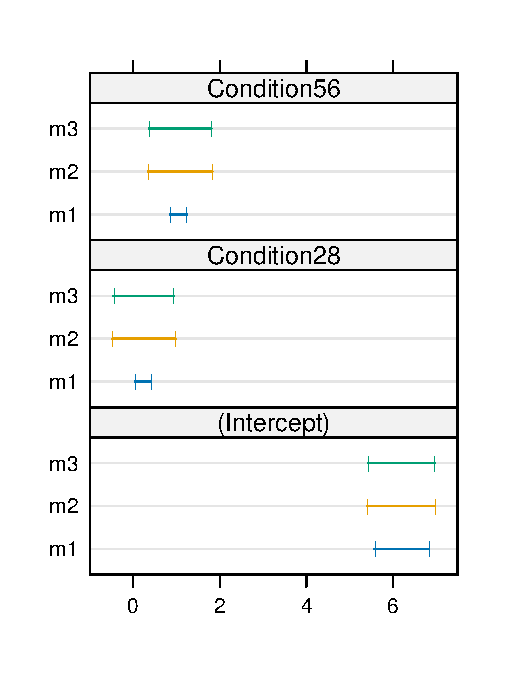
\includegraphics[scale=.6]{../figures/heal_ci}
    \end{column}
  \end{columns}
\end{frame}

\begin{frame}[fragile]{}
  \begin{block}{Exercise}
    \begin{itemize}
      \item Fit the models from the previous slide
      \item Profile the models with \texttt{profile(<model>)}
      \item Use the functions \texttt{xyplot()}, \texttt{densityplot()},
        \texttt{splom()} from the lattice package to take a closer look at the
        estimated random parameters
      \item Compare the three models with likelihood ratio tests
      \item What is the best model in your opinion?
    \end{itemize}
  \end{block}
\end{frame}

\begin{frame}[<+->]{Summary}
  \begin{itemize}
    \item When we use mixed-effects model to fit data, we need to make an
      informed choice about the random effects we include into the model
    \item Complex random effect structures can lead to convergence problems and
      random slopes are not always easy to estimate
    \item The random effects structure strongly influences the confidence
      intervals for the fixed effects which we are often interested in
    \item This is especially relevant in a confirmatory setting
    \item For some critical discussion of the healing paper and their choice of
      random effects see \citet{Gelman2024} and Gelman's blog post and
      discussion here:
      \url{https://statmodeling.stat.columbia.edu/2025/01/23/slopes/}
  \end{itemize}
\end{frame}

% \begin{frame}{Two-way repeated measures ANOVA}
%   \begin{align*}
%     &   y_{ijk} = \mu + \alpha_i + \beta_j + (\alpha\beta)_{ij} + \pi_k +
%         (\pi\alpha)_{ik} + (\pi\beta)_{jk} + \varepsilon_{ijk}\\
%     &  i = 1,\dots,p; j = 1,\dots,q; k = 1,\dots,n
%   \end{align*}
% 
%      with
%   \begin{align*}
%     \pi_k & \sim N(0, \sigma^2_{\pi})\\
%     (\pi\alpha)_{ik} & \sim N(0, \sigma^2_{\pi\alpha})\\
%     (\pi\beta)_{jk} & \sim N(0, \sigma^2_{\pi\beta})\\
%     \varepsilon_{ijk} & \sim N(0, \sigma^2_{\varepsilon})
%   \end{align*}
%      all random effects independent
% \vfill
% \end{frame}
% 
% \begin{frame}{From model to data}
%  \[
%    y_{ijk} = \mu + \alpha_i + \beta_j + (\alpha\beta)_{ij} + \pi_k +
%    (\pi\alpha)_{ik} + (\pi\beta)_{jk} + \varepsilon_{ijk}
%  \]
% 
% \centering
%   {\small
%   \begin{tabular}{crrrrrrrr}
%     \hline
%     subj & $\mu$ & $\alpha$ & $\beta$ & $(\alpha\beta)$ & $\pi$ & $(\pi\alpha)$ &
%     $(\pi\beta)$ & $\varepsilon$ \\
%     \hline
%     1 & $500$ & $ 10$ & $ 20$ & $-30$ & $0.82$ & $3.72$ & $-8.61$ & $-15.20$\\
%     1 & $500$ & $ 10$ & $-20$ & $ 30$ & $0.82$ & $3.72$ & $-0.64$ & $ 25.85$\\
%     1 & $500$ & $-10$ & $ 20$ & $ 30$ & $0.82$ & $4.98$ & $-8.61$ & $-12.13$\\
%     1 & $500$ & $-10$ & $-20$ & $-30$ & $0.82$ & $4.98$ & $-0.64$ & $ -3.02$\\
%     \vdots & & & & & & & & \\
%     30 & $500$ & $ 10$ & $ 20$ & $-30$ & $7.94$ & $3.72$ & $-8.61$ & $-4.14$\\
%     30 & $500$ & $ 10$ & $-20$ & $ 30$ & $7.94$ & $3.72$ & $-0.64$ & $-5.85$\\
%     30 & $500$ & $-10$ & $ 20$ & $ 30$ & $7.94$ & $4.98$ & $-8.61$ & $-5.63$\\
%     30 & $500$ & $-10$ & $-20$ & $-30$ & $7.94$ & $4.98$ & $-0.64$ & $28.02$\\
%     \hline
%   \end{tabular}
%   }
%   \begin{align*}
%     \sigma_{\pi}      & = 10 & \sigma_{\pi\alpha}   & =  7 \\
%     \sigma_{\pi\beta} & =  8 & \sigma_{\varepsilon} & = 15
%   \end{align*}
% \end{frame}
% 
% \begin{frame}{From model to data}
%       \[
%         y_{ijk} = \mu + \alpha_i + \beta_j + (\alpha\beta)_{ij} + \pi_k +
%         (\pi\alpha)_{ik} + (\pi\beta)_{jk} + \varepsilon_{ijk}
%       \]
% 
% \centering
%   \begin{tabular}{c|l|c}
%     \hline
%     subj &  & $y_{ijk}$ \\
%     \hline
%     1 & $500 + 10 + 20 - 30 + 0.82 + 3.72 - 8.61 - 15.20$ & 520.73\\
%     1 & $500 + 10 - 20 + 30 + 0.82 + 3.72 - 0.64 + 25.85$ & 499.75\\
%     1 & $500 - 10 + 20 + 30 + 0.82 + 4.98 - 8.61 - 12.13$ & 455.06\\
%     1 & $500 - 10 - 20 - 30 + 0.82 + 4.98 - 0.64 - 3.02$  & 522.14\\
%     \vdots &  & \vdots\\
%     30 & $500 + 10 + 20 - 30 + 7.94 + 3.72 - 8.61 - 4.14$  & 538.91\\
%     30 & $500 + 10 - 20 + 30 + 7.94 + 3.72 - 0.64 - 5.85$  & 475.17\\
%     30 & $500 - 10 + 20 + 30 + 7.94 + 4.98 - 8.61 - 5.63$  & 468.68\\
%     30 & $500 - 10 - 20 - 30 + 7.94 + 4.98 - 0.64 + 28.02$ & 560.30\\
%     \hline
%   \end{tabular}
%   \vfill
% \end{frame}
% 
% \begin{frame}{Matrix notation}
% {Effect coding}
% \[
%   \begin{pmatrix}
%     y_{111}\\
%     \vdots\\
%     y_{ijk}\\
%     \vdots\\
%     y_{22n}
%   \end{pmatrix}
% =
%   \begin{pmatrix}
%     1 & 1 & 1 & 1\\
%     \vdots & \vdots & \vdots & \vdots \\
%     1 & -1 & 1 & -1\\
%     \vdots & \vdots & \vdots & \vdots \\
%     1 & 1 & -1 & -1\\
%     \vdots & \vdots & \vdots & \vdots \\
%     1 & -1 & -1 & 1
%   \end{pmatrix}
% \times
%   \begin{pmatrix}
%     \mu\\
%     \alpha_2\\
%     \beta_2\\
%     (\alpha\beta)_{22}
%   \end{pmatrix}
% +
%   \begin{pmatrix}
%     1 & 0 & \dots & 0 & 0\\
%     \vdots & \vdots && \vdots & \vdots \\
%     0 & 1 & \dots & 0 & 0\\
%     \vdots & \vdots && \vdots & \vdots \\
%     0 & 0 & \dots & 1 & 0\\
%     \vdots & \vdots && \vdots & \vdots \\
%     0 & 0 & \dots & 0 & 1
%   \end{pmatrix}
% \times
%   \begin{pmatrix}
%     \pi_1\\
%     \vdots\\
%     \pi_n\\
%     (\pi\alpha)_{11}\\
%     \vdots\\
%     (\pi\alpha)_{2n}\\
%     (\pi\beta)_{11}\\
%     \vdots\\
%     (\pi\beta)_{2n}\\
%   \end{pmatrix}
% +
%   \begin{pmatrix}
%     e_{111}\\
%     \vdots\\
%     e_{ijk}\\
%     \vdots\\
%     e_{22n}
%   \end{pmatrix}
% \]
% \end{frame}
% 
% 
% \begin{frame}[fragile]{From model to data}
%   \begin{lstlisting}
% # Set effect coding 
% options(contrasts = c("contr.sum", "contr.poly"))
% 
% n <- 30
% 
% dat <- expand.grid(A = factor(c("a1", "a2")), 
%                    B = factor(c("b1", "b2")),
%                    subj = factor(1:n))
% 
% # Fixed effects (in ms), effect coding
% beta <- c(mu = 500, a2 = -10, b2 = -20, ab22 = -30)
% 
% # Model matrix 
% X <- model.matrix(~ A * B, dat)
%   \end{lstlisting}
% \end{frame}
% 
% \begin{frame}[fragile]{From model to data}
%   \begin{lstlisting}
% # Variance components (SD in ms)
% sp  <- 10
% spa <-  7
% spb <-  8
% se  <- 15
% 
% # Random effects
% u <- c(p = rnorm(n, sd = sp), 
%        pa = rnorm(2 * n, sd = spa), 
%        pb = rnorm(2 * n, sd = spb))
% 
% Z <- model.matrix(~ 0 + subj + subj:A + subj:B, dat, 
%   contrasts.arg = lapply(dat, contrasts, contrasts = FALSE))
%   \end{lstlisting}
% \end{frame}
% 
% 
% \begin{frame}[fragile]{From model to data}
% \begin{lstlisting}
% # Calculate dependent variable
% dat$RT <- X %*% beta + Z %*% u + rnorm(2*2*n, sd=se)
% 
% # Look at simulated data
% with(dat, interaction.plot(A, B, RT, type = "b", pch = c(21, 16),
%   ylim = c(400, 600)))
% \end{lstlisting}
%   \nocite{Wickelmaier2022}
% \end{frame}

\appendix

\begin{frame}[allowframebreaks]{References}
%\begin{frame}{References}
  %\renewcommand{\bibfont}{\footnotesize}
  \printbibliography
  %\vfill
\end{frame}

\end{document}

